%
% etraeger.tex
%
% (c) 2023 Prof Dr Andreas Müller
%
\begin{figure}
\centering
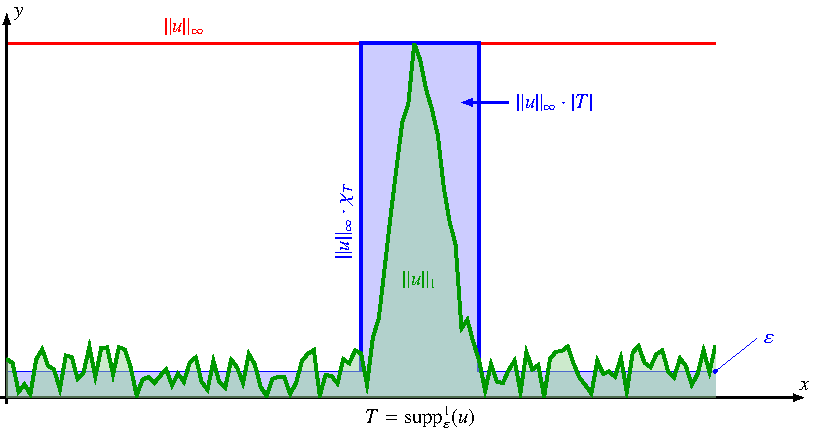
\includegraphics{chapters/060-diskret/images/etraeger.pdf}
\caption{$(\varepsilon,1)$-Träger als Mass für die Lokalsierung
einer Funktion.
Im Bereich der Menge $T$ ist die $L^1$-Norm des so gross, dass
die $L^1$-Norm auf dem Komplement von $L^1$ nur das $\varepsilon$-fache
der $L^1$-Norm $\|u\|_1$ ist.
\label{buch:diskret:unschaerfe:fig:etraeger}}
\end{figure}%
